\chapter{Targeted Transcriptome}\label{ch: targeted_transcriptome}
\label{targetedmousetranscriptome}

%https://www.nature.com/articles/s41467-020-17009-7#Sec14

\section{Introduction}
One current limitation of whole transcriptome sequencing is the low coverage/sequencing depth achieved per gene due to the distribution of reads across the whole transcriptome. Consequently, while whole transcriptome sequencing allows identification of novel genes (genes not previously annotated to the genome) and novel isoforms, it may not detect isoforms particularly those of low expression resulting in many false negatives. This can be circumvented by the use of target capture, which enriches a selective panel of genes that are then only sequenced. Multiple samples can further be pooled and sequenced together by barcoding samples at cDNA synthesis, which simplifies laboratory workflow and minimises associated sequencing costs.

%[Other methods of Targeted Sequencing i.e. CRISPR]

%Advantages of targeted transcriptomics vs whole transcriptomics; resources in Targeted Transcriptomics paper; Literature Review 
%List of relevance of AD genes

%Single cell RNA-Sequencing identified subsets of protective microglia, referred as disease-associated microglia (DAM), with a characteristic transcriptional activation profile: Trem2-dependent upregulation of phagocytic-related genes, essential for A$\beta$ clearance\cite{Keren-Shaul2017}. 

%Single cell RNA-Sequencing of mouse also revealed two main activated states (reactive) of microglia, activated response microglia (ARM) characterised by upregulated expression of immune cells, and interferon response microglia (IRM) characterised by upregulated expression of innate immune response and interferon response pathway \cite{Frigerio2019}. ARM was enriched with GWAS AD risk genes, with upregulation of \textit{Trem2} and downregulation of \textit{Bin1,Cd33,Picalm}. ARM also promote \textit{Apoe} expression in microglia, whereby deletion of \textit{APOE} ablated ARM expression and density of microglia around amyloid deposits \cite{Frigerio2019} 
%Single cell RNA-Sequencing of AD prefrontal cortex further revealed cell-specific response with upregulation of microglial-expressed genes, such as \textit{Trem2} and \textit{PICALM}, that positively correlately with AD pathology in micrologia \cite{Mathys2019}.
%Structural crystallography studies of mutant TREM2 proteins reveal that AD-associated risk variants were localised to the receptor's functional surface, thereby reducing ligand binding affinity\cite{Kober2016}, and modulate TREM2 signalling \cite{Wang2015a}.
%Mouse-specific microglial expression signatures are not readily recapitulated in human microglia from recent studies using single-nucleus RNA-sequencing (snRNA-seq) \cite{Thrupp2020,Olah2020} with only a low overlap of activation genes reported \cite{Grubman2019,Mathys2019} - these inconsistencies may be reflective of the limtations of snRNA-seq to capture human microlglial activation genes \cite{Thrupp2020}.
%https://journals.lww.com/co-neurology/Fulltext/2021/04000/The_role_of_innate_immune_genes_in_Alzheimer_s.13.aspx#:~:text=Neuroinflammation%20is%20as%20an%20innate,role%20in%20Alzheimer's%20disease%20pathogenesis
%https://www.nature.com/articles/s41598-020-75057-x


\section{Methods}

\subsection{Samples}
Extracted RNA from mouse entorhinal cortex of wild-type and transgenic rTg4510 mice was sequenced on the PacBio's Sequel (n = 24, Table \ref{tab:mouse_samples_sequenced}), a subset of which were also sequenced on the Oxford Nanopore's MinION (n = 18, Table \ref{tab:mouse_samples_sequenced}). Three biological replicates were selected at each age (2, 4, 6 and 8 months) across wild-type and transgenic mice, multiplexed with barcodes (listed in \cref{tab:barcode_primers}) and sequenced as three batches.

\subsection{Library preparation and sequencing}
Following the Iso-Seq lab protocol (as described in \cref{chap:isoseq_labpipeline}), 200ng RNA from each sample was primed for first strand cDNA synthesis (\cref{section:ch2_cDNA_synthesis_explanation}) with specific oligo-dT barcodes and amplified using PCR with 14 cycles (\cref{fig:isoseq_targeted_pccresults}, \cref{section:ch2_PCR_explanation}). Following purification with 0.4X and 1X AMPure PB beads, the two fractions were then recombined at equimolar quantities, and samples were subsequently combined at equimolar quantities according to each batch. Enrichment for target genes with IDT hybridisation capture was then performed for each batch (described in \cref{section:ch2_targetcapture_explanation}) using custom-designed probes (summarised in \cref{tab:mouse_probes}). Following successful target capture and library preparation (depicted in \cref{fig:isoseq_targeted_libresults}), sequencing was performed for each batch on the PacBio Sequel using a 1M SMRT cell. RNA from the same samples (n = 24) was also prepared with TruSeq Stranded mRNA Sample Prep Kit (Illumina) and subjected to 125bp paired-end sequencing using a HiSeq2500 (Illumina), and used as junction support of the long reads. 

\subsection{SMRT sequencing QC and data processing}
Processing of raw reads were performed using the Iso-Seq bioinformatics pipeline (outlined in \cref{section:isoseq_bioinformatics}), and is similar to the whole transcriptomics data processing with the exception of demultiplexing samples at \textit{Lima} with barcodes. Briefly, CCS reads were generated for each batch and demultiplexed for each sample. Full-length reads from each sample were then merged and collapsed to unique isoforms with \textit{Cupcake}, which were mapped to mouse reference genome (mm10) using \textit{Minimap2} and annotated with \textit{SQANTI3}. Partial isoforms as a consequence of 5'degradation were filtered out using \textit{TAMA}'s script (tama\_remove\_fragment\_models.py) with default parameters. Full-length Iso-Seq read counts from each individual sample were extracted from \textit{Cupcake's} read\_stat.txt file.

\begin{landscape}
\begin{table}[]
		\resizebox{1.5\textwidth}{!}{%
	\begin{tabular}{@{}cccccccccc@{}}
		\toprule
		\multicolumn{6}{c}{\multirow{2}{*}{\begin{tabular}[c]{@{}c@{}}Sample   \\ demographics\end{tabular}}} &
		\multicolumn{4}{c}{Sequencing Platform} \\ \cmidrule(l){7-10} 
		\multicolumn{6}{c}{}                      & \multicolumn{2}{c}{PacBio Iso-Seq} & \multicolumn{2}{c}{Oxford Nanopore} \\ \midrule
		Sample &
		Phenotype &
		Age (Months) &
		RIN &
		\begin{tabular}[c]{@{}c@{}}Concentration\\ (ng/ul)\end{tabular} &
		\begin{tabular}[c]{@{}c@{}}Batch \\ (Barcodes)\end{tabular} &
		\begin{tabular}[c]{@{}c@{}}Whole \\ Transcriptome\end{tabular} &
		\begin{tabular}[c]{@{}c@{}}Targeted\\  Transcriptome\end{tabular} &
		\begin{tabular}[c]{@{}c@{}}Whole \\ Transcriptome\end{tabular} &
		\begin{tabular}[c]{@{}c@{}}Targeted \\ Transcriptome\end{tabular} \\ \midrule
		K19 & WT & 4 & 8.8 & 236  & 1 (PB\_BC\_1) &                 & X               &                  &                  \\
		K23 & WT & 8 & 9.1 & 143  & 1 (PB\_BC\_2) & X               & X               &                  &                  \\
		K21 & WT & 6 & 9   & 138  & 1 (PB\_BC\_3) &                 & X               &                  &                  \\
		K18 & TG & 2 & 8.8 & 136  & 1 (PB\_BC\_4) & X               & X               & X                &                  \\
		K20 & TG & 4 & 9.1 & 80.4 & 1 (PB\_BC\_5) &                 & X               &                  &                  \\
		K17 & WT & 2 & 9.2 & 77.1 & 1 (PB\_BC\_6) & X               & X               &                  &                  \\
		S19 & WT & 4 & 9.1 & 84.9 & 2 (PB\_BC\_1) &                 & X               &                  & X                \\
		K24 & TG & 8 & 9.2 & 65.4 & 2 (PB\_BC\_2) & X               & X               &                  & X                \\
		L22 & TG & 8 & 8.7 & 68.6 & 2 (PB\_BC\_3) & X               & X               &                  & X                \\
		M21 & WT & 2 & 9.2 & 72.3 & 2 (PB\_BC\_4) & X               & X               & X                & X                \\
		O18 & TG & 2 & 8.9 & 115  & 2 (PB\_BC\_5) & X               & X               &                  & X                \\
		O23 & WT & 8 & 9   & 91.8 & 2 (PB\_BC\_6) & X               & X               &                  & X                \\
		O22 & TG & 6 & 9.1 & 83.5 & 2 (PB\_BC\_7) &                 & X               &                  & X                \\
		P19 & WT & 6 & 8.9 & 92.2 & 2 (PB\_BC\_8) &                 & X               &                  & X                \\
		T20 & TG & 6 & 9   & 68.7 & 2 (PB\_BC\_9) &                 & X               &                  & X                \\
		Q20 & TG & 8 & 8.6 & 99.7 & 3 (PB\_BC\_1) & X               & X               &                  & X                \\
		Q21 & WT & 2 & 9.2 & 83.3 & 3 (PB\_BC\_2) & X               & X               &                  & X                \\
		S18 & TG & 2 & 8.9 & 115  & 3 (PB\_BC\_3) & X               & X               &                  & X                \\
		S23 & WT & 8 & 9.1 & 95.5 & 3 (PB\_BC\_4) & X               & X               &                  & X                \\
		Q18 & TG & 6 & 8.8 & 87.2 & 3 (PB\_BC\_5) &                 & X               &                  & X                \\
		Q17 & WT & 6 & 8.7 & 85.8 & 3 (PB\_BC\_6) &                 & X               &                  & X                \\
		L18 & TG & 4 & 8.8 & 145  & 3 (PB\_BC\_7) &                 & X               &                  & X                \\
		Q23 & WT & 4 & 9   & 70.8 & 3 (PB\_BC\_8) &                 & X               &                  & X                \\
		T18 & TG & 4 & 9   & 85   & 3 (PB\_BC\_9) &                 & X               &                  & X                \\ \bottomrule
	\end{tabular}%
}
\captionsetup{width=1.5\textwidth}
\caption[Mouse rTg4510 samples sequenced using whole and targeted transcriptome approach with PacBio Iso-Seq and ONT nanopore sequencing]%
{Mouse rTg4510 samples sequenced using whole and targeted transcriptome approach with PacBio Iso-Seq and ONT nanopore sequencing}
\label{tab:mouse_samples_sequenced}
\end{table}
\end{landscape}


\begin{table}[ht]
	\begin{tabular}{@{}cccccc@{}}
		\toprule
		Target &
		\begin{tabular}[c]{@{}c@{}}Number \\ of \\ Probes\end{tabular} &
		\begin{tabular}[c]{@{}c@{}}Genome \\ Co-ordinates\end{tabular} &
		Strand &
		\begin{tabular}[c]{@{}c@{}}Full\\  Region\\  (bp)\end{tabular} &
		\begin{tabular}[c]{@{}c@{}}Exons inc UTR \\ (bp)\end{tabular} \\ \midrule
		ABCA1  & 56         & chr  4 : 53030670 -   53160014    & - & 129,107 & 10,260 \\
		ABCA7  & 47         & chr  10 : 79997615 -   80015572   & + & 17,958  & 6,594  \\
		ANK1   & 52         & chr  8 : 22974836 -   23150497    & + & 175,662 & 9,018  \\
		APOE   & 5          & chr  7 : 19696125 -   19699285    & - & 2,923   & 1,251  \\
		APP    & 20         & chr  16 : 84954317 -   85173826   & - & 219,272 & 3,357  \\
		BIN1   & 20         & chr  18 : 32377217 -   32435740   & + & 58,524  & 2,455  \\
		CD33   & 9          & chr  7 : 43528610 -   43533290    & - & 5,716   & 2,571  \\
		CLU    & 9          & chr  14 : 65968483 -   65981545   & + & 13,063  & 1,808  \\
		FUS    & 16         & chr  7 : 127967479 -   127982032  & + & 14,554  & 1,845  \\
		FYN    & 18         & chr  10 : 39369799 -   39565381   & + & 195,583 & 3,692  \\
		MAPT   & 23         & chr  11 : 104231436 -   104332096 & + & 100,661 & 5,387  \\
		PICALM & 24         & chr  7 : 90130232 -   90209447    & + & 79,216  & 4,174  \\
		PTK2B  & 32         & chr  14 : 66153138 -   66281171   & - & 127,796 & 4,034  \\
		RHBDF2 & 21         & chr  11 : 116598082 -   116627138 & - & 28,855  & 3,934  \\
		SNCA   & 7          & chr  6 : 60731454 -   60829974    & - & 98,283  & 1,463  \\
		SORL1  & 48         & chr  9 : 41968370 -   42124408    & - & 155,801 & 6,938  \\
		TARDBP & 15         & chr  4 : 148612263 -   148627115  & - & 14,615  & 7,454  \\
		TREM2  & 5          & chr  17 : 48346401 -   48352276   & + & 5,876   & 1,146  \\
		TRPA1  & 28         & chr  1 : 14872529 -   14918981    & - & 46,215  & 4,263  \\
		VGF    & 9          & chr  5 : 137030295 -   137033351  & + & 3,057   & 2,553  \\
		& Total: 464 &                                   &   &         &        \\ \bottomrule
	\end{tabular}
\caption[Mouse probes for enrichment of AD-associated target genes]%
{\textbf{Mouse probes for enrichment of AD-associated target genes}. For target enrichment and subsequent sequencing, probes were designed and curated to 20 AD-associated genes (as detailed in \cref{section:ch2_targetcapture_explanation})}
\label{tab:mouse_probes}
\end{table}


\begin{figure}[htp]
	\centering
	\vspace{20pt}
	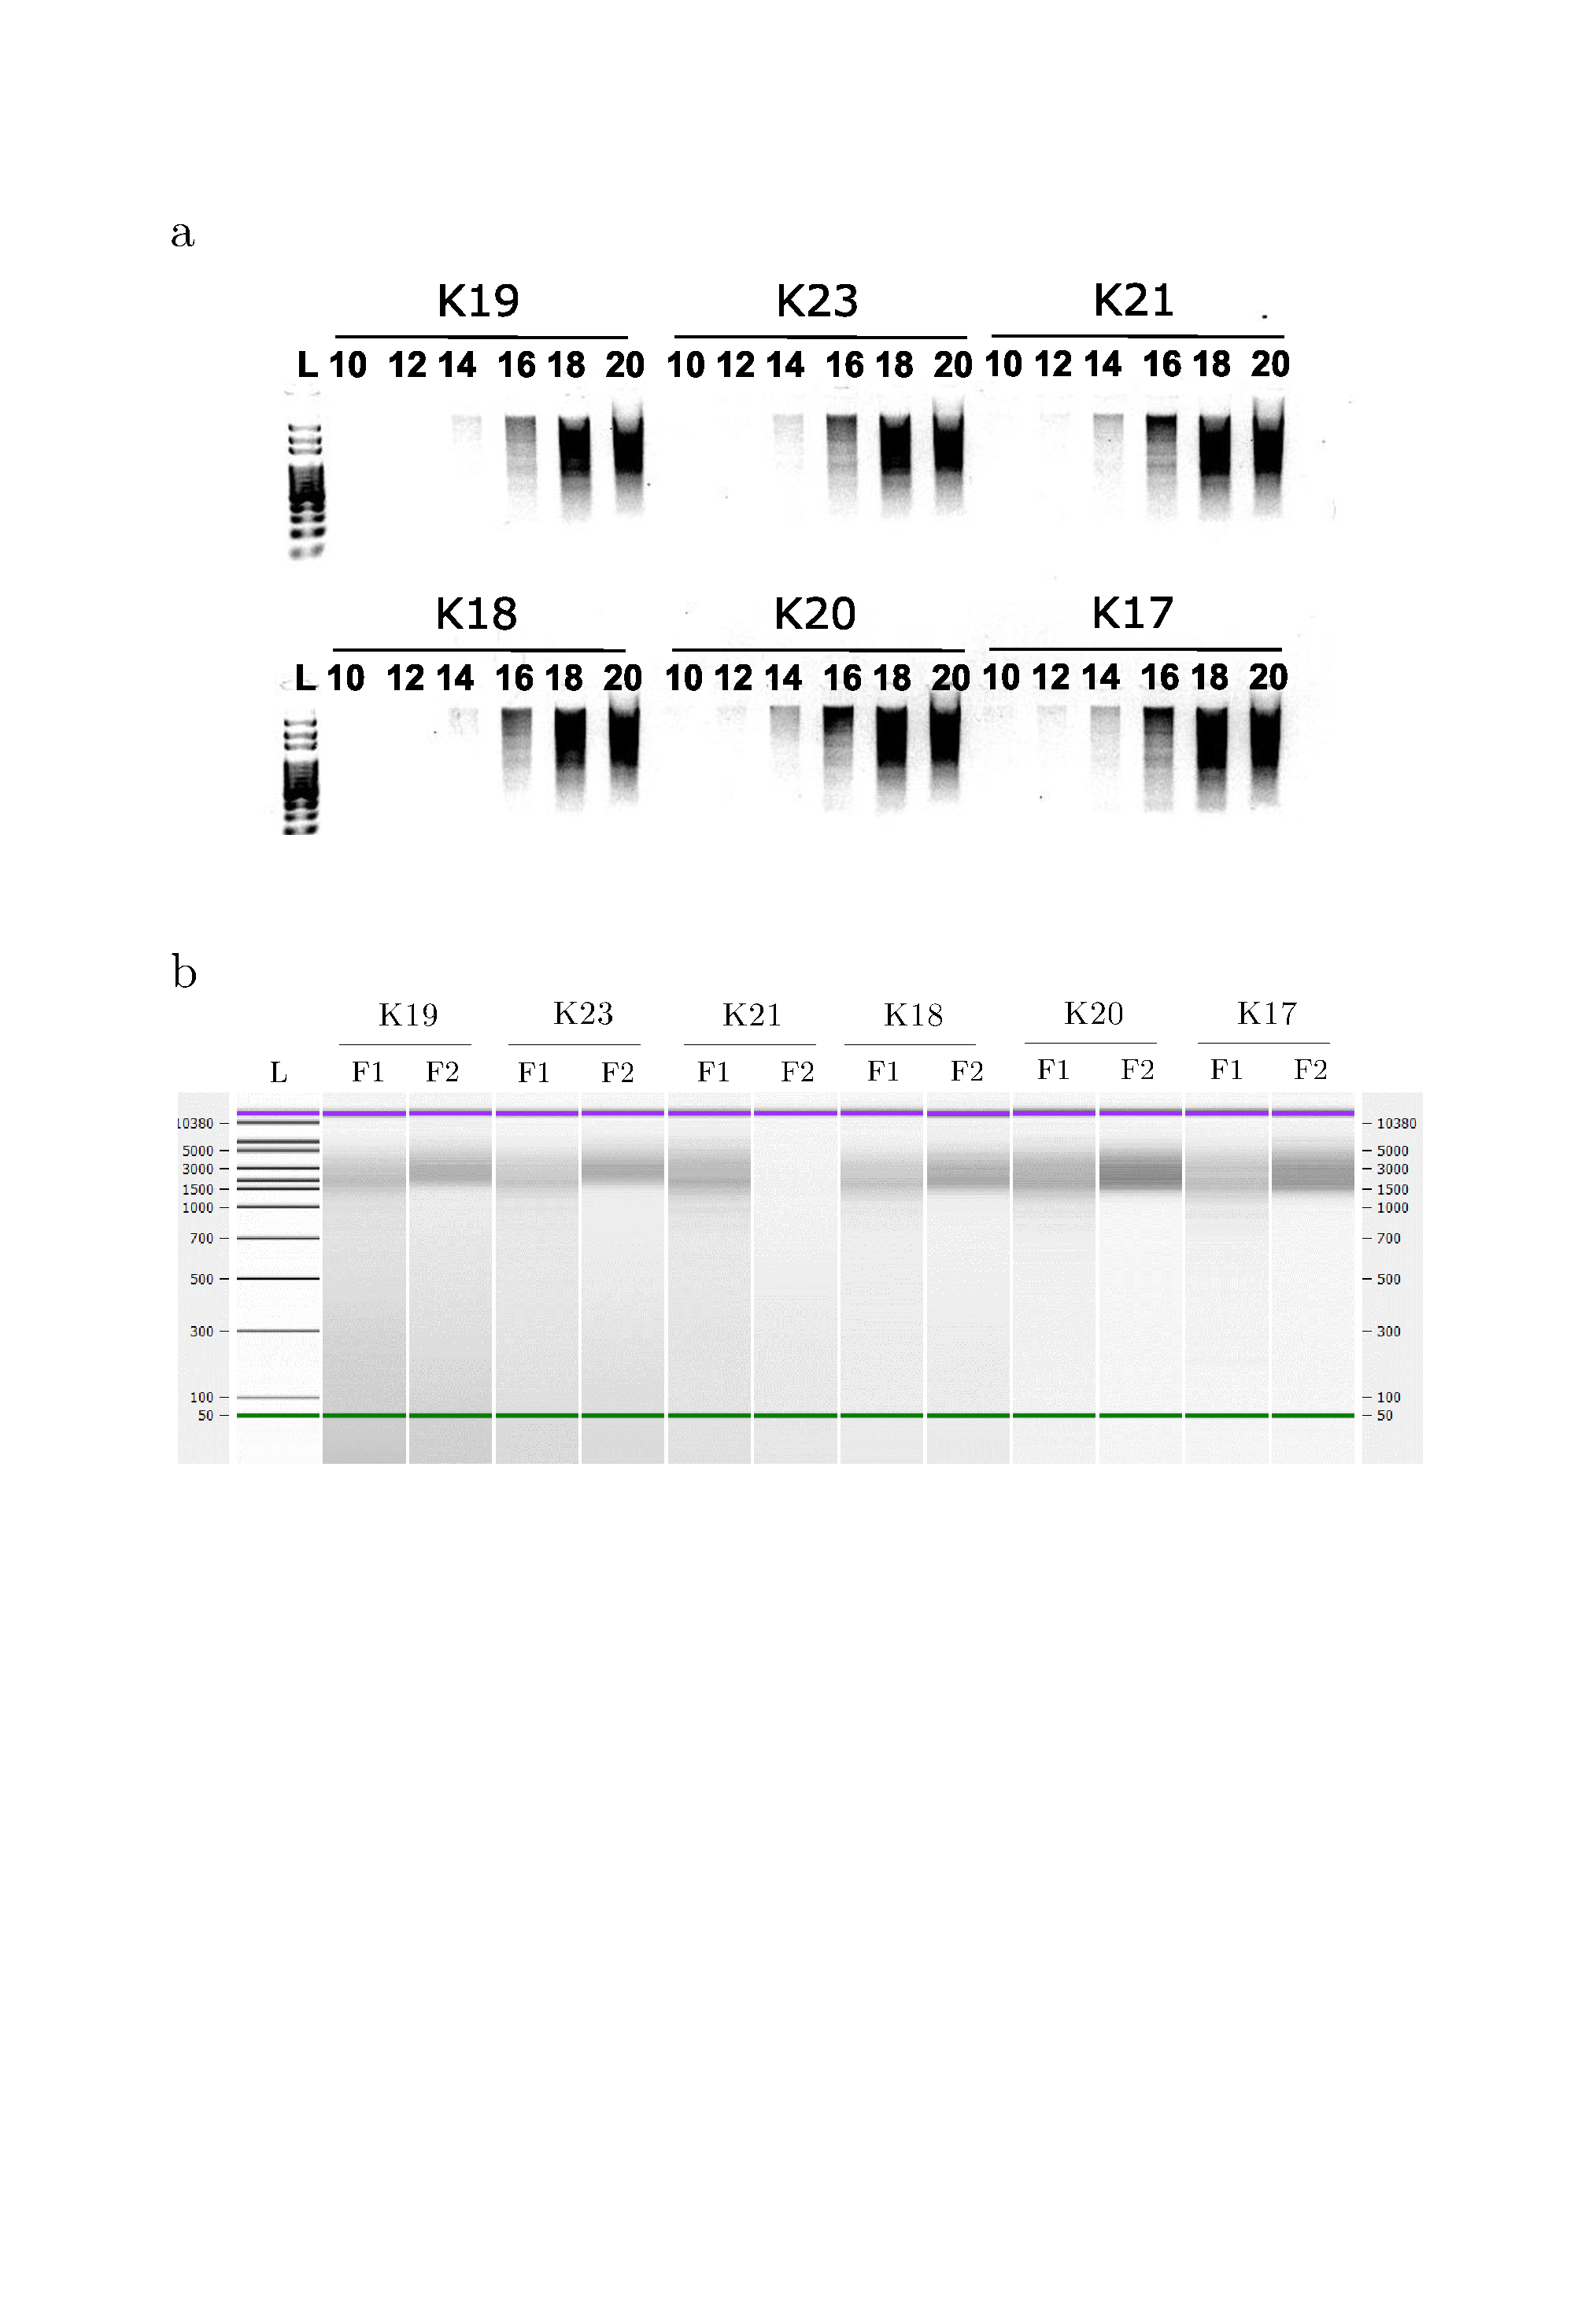
\includegraphics[page=1,trim={0 16cm 0 4cm},clip,scale = 0.45]{Figures/TargetedLabResults.pdf}
	\captionsetup{width=0.95\textwidth}
	\caption[Iso-Seq Targeted Transcriptome - cDNA amplification and purification]%
	{\textbf{The first stage between the targeted and whole transcriptome sequencing is the same with samples typically amplified using 14 cycles followed by enrichment of high molecular weight cDNA in Fraction 2: a)} Like whole transcriptome sequencing, samples were amplified using 14 cycles (Figure \ref{fig:isoseq_whole_pccresults}) whereby cycles below generated insufficient cDNA and cycles above showed signs of over-amplification. The samples shown here (K19, K23, K21, K18, K20, K17) were multiplexed and sequenced in Batch 1 (see Table \ref{tab:mouse_samples_sequenced}. Ladder (L) shown is 100bp DNA ladder. \textbf{b)} Similar to whole transcriptome sequencing, amplified cDNA was further divided into two fractions (denoted here as F1 and F2) and purified with 1X (F1) and 0.4X (F2) AMPure beads. As shown in the Bioanalyzer gel, there was an enrichment of higher-molecular weight cDNA in Fraction 2 compared to Fraction 1 across all the samples (with the exception of Sample K21 with loss of Fraction 2). Green and purple line represent the lower marker at 50bp and the upper marker at 17kb respectively. F1 - Fraction 1 containing cDNA purified with 1X AMPure beads; F2 - Fraction 2 containing cDNA purified with 0.4X AMPure beads.}
	\label{fig:isoseq_targeted_pccresults}
\end{figure}


\begin{figure}[!htp]
	\centering
	\vspace{20pt}
	\includegraphics[page=2,trim={0 14cm 3cm 1cm},clip,scale = 0.45]{Figures/TargetedLabResults.pdf}
	\captionsetup{width=0.95\textwidth}
	\caption[Iso-Seq Targeted Transcriptome - Target Capture and library preparation]%
	{\textbf{Successful target capture and library preparation across all batches, as shown by enrichment of transcripts with specific lengths:} \textbf{a)} and \textbf{c)} are Bioanalyzer electropherogram traces of Batch 1 (n = 6) and Batch 2 (n = 9) respectively after enrichment of cDNA with selective IDT probes (Section \ref{section:ch2_targetcapture_explanation}). \textbf{b)}, \textbf{d)} and \textbf{f)} are Bioanalyzer electropherogram traces of Batch 1, 2 and 3 respectively after library preparation (denoted here as "Final", Section \ref{section:ch2_smrtbelltemplate_explanation}. \textbf{e)} An overlay of Batch 2 after target capture and library preparation. 
	\\
	\\
	As can be seen across all figures, target capture appears to be successful with detected peaks, reflecting enrichment of target transcripts with specific lengths, which differs from the broad peaks that are evident in whole transcriptome sequencing (Figure \ref{fig:isoseq_whole_bioresults}). Library preparation with ligation of SMRT bell templates retained these targeted transcripts with good peak overlay, as seen in figure e). The difference in peak height (i.e. cDNA quantity) between target capture and library preparation is due to a difference in input cDNA concentration when running Bioanalyzer - input cDNA after library preparation was diluted with a 1:5 dilution factor to maximise amount of cDNA available for sequencing, whereas input cDNA after target capture was not diluted.}  
	\label{fig:isoseq_targeted_libresults}
\end{figure}


\subsection{Transcriptome Annotation and Iso-Seq Quantification}
Isoforms were annotated with \textit{SQANTI3} in combination with mouse reference gene annotations (mouse GENCODE, vm22), FANTOM5 CAGE peaks and \textit{STAR}-aligned RNA-Seq junctions, and were classified as either FSM, ISM, NIC, NNC, antisense, fusion, and intergenic (described in \cref{section: sqanti_annotations}). ISM isoforms were assumed as partial products of longer FSM isoforms, and associated read counts were aggregated.   

\newpage
\section{Results}
\subsection{Run performance and sequencing metrics}
Following library preparation and SMRT sequencing, a total of XXGb (s.d = XXGb) were obtained (Table \ref{tab:targeted_mouse_run_output}). Of note, 6 samples were first trialled and multiplexed in Batch 1 to determine the yield output and coverage depth - PacBio recommends starting with 4 - 8 samples for multiplexing. Having noticed that an average yield output (24Gb) with a high off-target sequencing, implicating saturation of target genes with 6 samples, the number was increased to 9 samples in Batch 2 and Batch 3. Despite more samples, the sequencing run for Batch 2 and 3, performed by Exeter's Seqeuncing Service, had a poor loading rate (38.1\% P1 of Batch 3 vs 71\% of Batch 1) and low subsequent yield. The samples were also potentially degraded after having been stored in -20\textdegree C for over 6 months due to Covid-19 lockdown. 

The yield difference between the first and last two batches was evident in the number of CCS reads (total = 996K; Batch 1 = 469K, Batch 2 = 306K, Batch 3 = 2221K Figure \ref{fig:isoseq_targeted_run_output}a) and FLNC reads (total = 930K; Batch 1 = 399K, Batch 2 = 275K, Batch 3 = 256K, Figure \ref{fig:isoseq_targeted_run_output}a) generated, after applying the bioinformatics Iso-Seq pipeline (same as the whole transcriptome approach with the exception of removing barcodes rather than general primers). However, calculation of the on-target rate suggested that while Batch 2 and 3 had lower output yield, the coverage of target genes was significantly greater than Batch 1 due to the increased sample size (mean rate in Batch 1 = 34.5\%; mean rate in Batch 2 = 46.2\%; mean rate in Batch 3: 42.9\%, Figure \ref{fig:isoseq_targeted_rate}). The on-target rate is defined as the proportion of mapped transcripts with sequences overlapping at least one target probe. 
%Off-target 

In addition to batch variability, the number of full-length transcripts obtained per sample varied within each batch (Figure \ref{fig:isoseq_targeted_run_output}b). This variability was not associated with RIN (corr = 0.147, P = 0.492, Spearman's rank) and is unlikely to be due to library preparation, given that samples were pooled in equal molarity during target capture. However, there was no significant difference in the number of full-length transcripts between WT and TG across the batched runs (Wilcoxon rank sum test, W = 73, P = 0.977, Figure \ref{fig:isoseq_targeted_run_output}c). 

\begin{landscape}
	\begin{table}[]
		\resizebox{1.5\textwidth}{!}{%
			\begin{tabular}{@{}cccccccccccccccccccl@{}}
				\toprule
				\multirow{3}{*}{Sample} &
				\multirow{3}{*}{\begin{tabular}[c]{@{}c@{}}Total \\ Bases \\ (GB)\end{tabular}} &
				\multirow{3}{*}{\begin{tabular}[c]{@{}c@{}}Polymerase\\ Reads\end{tabular}} &
				\multicolumn{6}{c}{Read   Length} &
				\multicolumn{3}{c}{Productivity} &
				\multicolumn{4}{c}{Control} &
				\multirow{3}{*}{\begin{tabular}[c]{@{}c@{}}Local \\ Base \\ Rate\end{tabular}} &
				\multicolumn{2}{c}{Template} &
				\multicolumn{1}{c}{\multirow{3}{*}{Notes}} \\ \cmidrule(lr){4-16} \cmidrule(lr){18-19}
				&
				&
				&
				\multicolumn{2}{c}{Polymerase} &
				\multicolumn{2}{c}{Subread} &
				\multicolumn{2}{c}{Insert} &
				\multirow{2}{*}{P0} &
				\multirow{2}{*}{P1} &
				\multirow{2}{*}{P2} &
				\multirow{2}{*}{\begin{tabular}[c]{@{}c@{}}Total   \\ Reads\end{tabular}} &
				\multirow{2}{*}{\begin{tabular}[c]{@{}c@{}}Read \\ Length\\  Mean\end{tabular}} &
				\multicolumn{2}{c}{Concordance} &
				&
				\multirow{2}{*}{\begin{tabular}[c]{@{}c@{}}Adapter   \\ Dimer \\ (0-10bp)\end{tabular}} &
				\multirow{2}{*}{\begin{tabular}[c]{@{}c@{}}Short \\ Insert \\ (11-100bp)\end{tabular}} &
				\multicolumn{1}{c}{} \\ \cmidrule(lr){4-9} \cmidrule(lr){15-16}
				&
				&
				&
				Mean &
				N50 &
				Mean &
				N50 &
				Mean &
				N50 &
				&
				&
				&
				&
				&
				Mean &
				Mode &
				&
				&
				&
				\multicolumn{1}{c}{} \\ \midrule
				Batch 1 &
				24.2 &
				712250 &
				34016 &
				70473 &
				1402 &
				1852 &
				3024 &
				3808 &
				\begin{tabular}[c]{@{}c@{}}4.62\% \\ (46613)\end{tabular} &
				\begin{tabular}[c]{@{}c@{}}71.58\%\\  (722026)\end{tabular} &
				\begin{tabular}[c]{@{}c@{}}24.76\% \\ (249707)\end{tabular} &
				9,690 &
				31,505 &
				0.84 &
				0.87 &
				2.31 &
				0 &
				0 &
				Sequenced in November 2019 \\
				Batch 2 &
				&
				&
				&
				&
				&
				&
				&
				&
				&
				&
				&
				&
				&
				&
				&
				&
				&
				&
				\multirow{2}{*}{\begin{tabular}[c]{@{}l@{}}Sequenced in July 2020\\ Samples were kept at -20 for over 9months. \\ Sequel broke down mid-run.  \\ Sequencing was prepared by Exeter's Sequencing Services\\ \\ \end{tabular}} \\
				Batch 3 &
				19.3 &
				383292 &
				50472 &
				100255 &
				1557 &
				2017 &
				3158 &
				3898 &
				\begin{tabular}[c]{@{}c@{}}18.68\% \\ (189549)\end{tabular} &
				\begin{tabular}[c]{@{}c@{}}38.11\%\\  (386743)\end{tabular} &
				\begin{tabular}[c]{@{}c@{}}43.56\% \\ (442054)\end{tabular} &
				3,440 &
				52,533 &
				0.85 &
				0.87 &
				2.86 &
				0 &
				0 &
				\\ \bottomrule
			\end{tabular}%
		}
		\captionsetup{width=1.5\textwidth}
		\caption[Run Yield Output from Targeted Transcriptome Iso-Seq of Tg4510]%
		{Iso-Seq run yield for each batch of Tg4510 mouse samples sequenced using targeted transcriptome approach}
		\label{tab:targeted_mouse_run_output}
	\end{table}
\end{landscape}

\begin{figure}[!htp]
	\begin{center}
		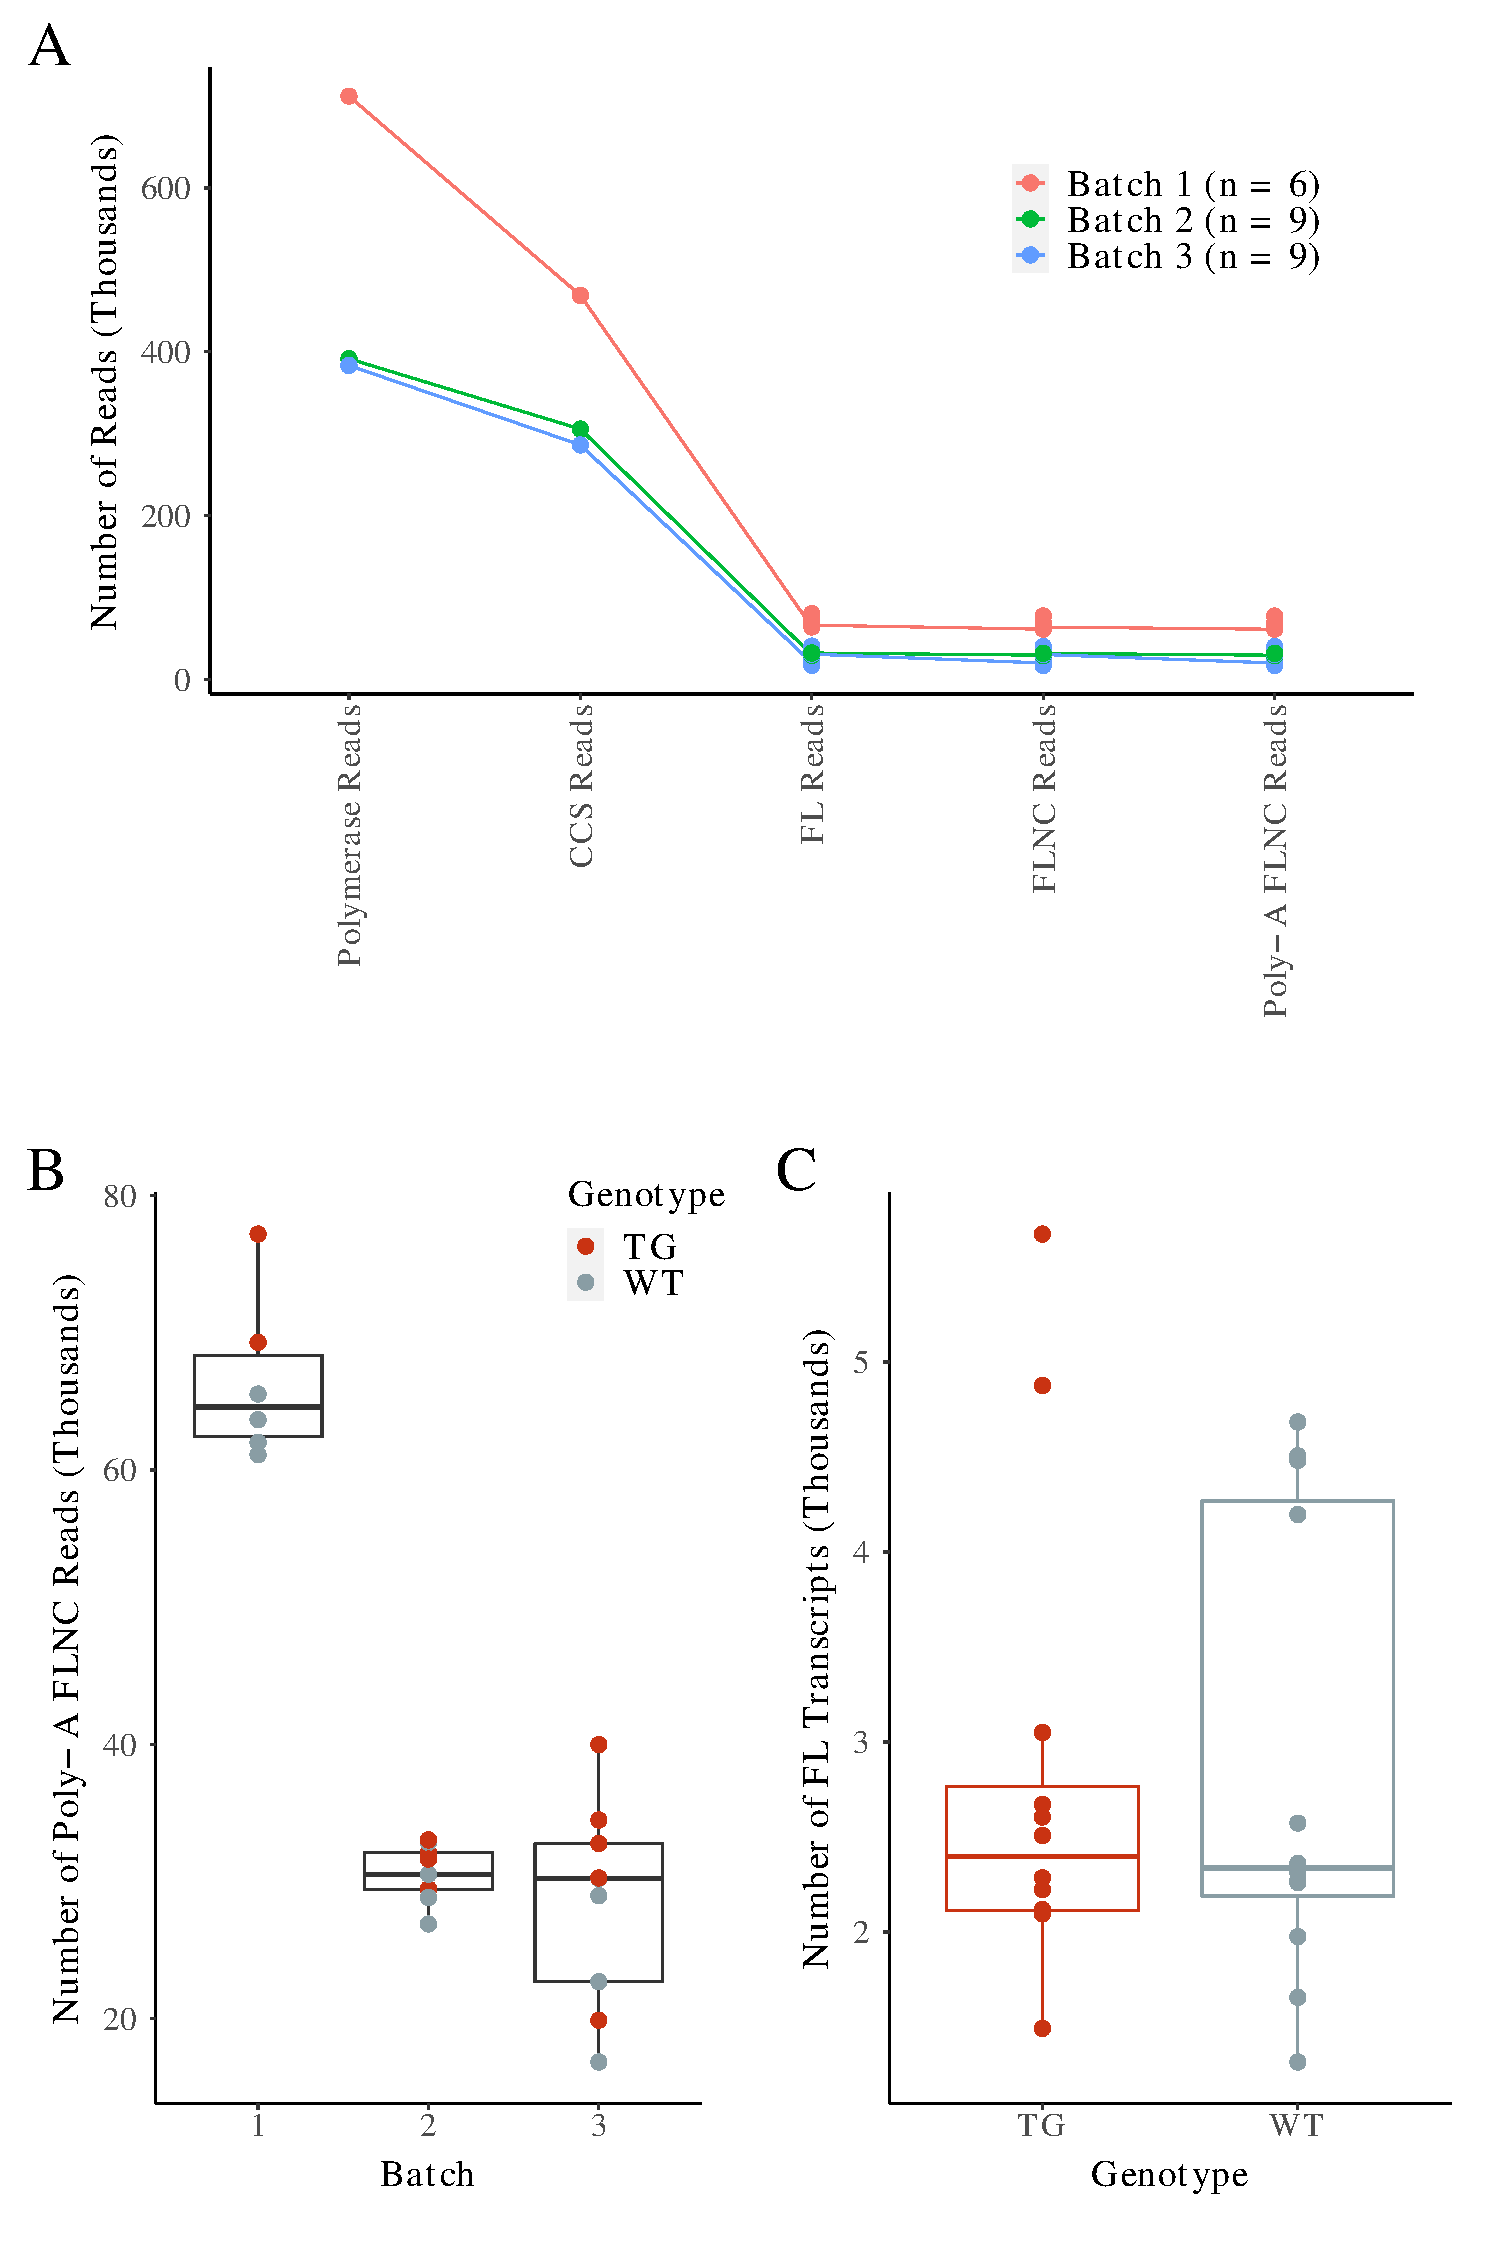
\includegraphics[page=1,trim={0 1cm 0 0},clip,scale = 0.55]{Figures/TargetedTranscriptome.pdf}
	\end{center}
	\captionsetup{width=0.95\textwidth}
	\caption[Targeted Transcriptome Iso-seq run performance]%
	{\textbf{Despite batch variability in targeted transcriptome sequencing, no difference in the number of full-length transcripts was observed between wildtype and transgenic mice}. \textbf{a)} Samples (n = 24) were multiplexed and sequenced in three runs (Batch 1, 2 and 3) with varied performance, as indicated by the number of polymerase reads through to poly-A FLNC reads. In the bioinformatics pipeline, the samples were demultiplexed and individually processed after generation of CCS reads from each run. \textbf{b)} Sample variability within each batch was observed from the number of poly-A FLNC reads generated. However, \textbf{c)} no statistical difference was observed in the overall number of full-length transcripts detected between wild-type and transgenic. Full-length transcripts were collapsed from poly-A FLNC reads in Iso-Seq Cluster. CCS - Circular Consensus Sequence, FLNC - Full-Length Non-Concatemer, FL - Full-Length, WT - Wild-type, TG - Transgenic}
	\label{fig:isoseq_targeted_run_output}
\end{figure}

\begin{figure}[!htp]
	\begin{center}
		\includegraphics[page=2,trim={0 25cm 0 0},clip,scale = 0.55]{Figures/TargetedTranscriptome.pdf}
	\end{center}
	\captionsetup{width=0.95\textwidth}
	\caption[On-Target rate in Transcriptome Iso-Seq runs]%
	{\textbf{Coverage of target genes was greater in Batch 2 and 3 than Batch 1 due to more samples multiplexed and sequenced}. Samples (n = 24) were multiplexed and sequenced in three runs (Batch 1 = 6 samples, Batch 2 = 9 samples, Batch 3 = 9 samples). Despite lower run yield output (\ref{tab:targeted_mouse_run_output}), Batch 2 and Batch 3 had a higher on-target rate, which refers to the proportion full-length transcripts associated with target genes. A difference in the on-target rate between wild-type and transgenic samples was observed in Batch 1, which is a likely reflection of the sample variability in sequencing (Figure \ref{fig:isoseq_targeted_run_output}b). WT - Wild-type, TG - Transgenic}
	\label{fig:isoseq_targeted_rate}
\end{figure}


%Following library preparation and nanopore sequencing (Chapter X), a total of 28.54M reads (39.68Gb) were generated across two flow cells and a total of 22.8M (80\%) reads were successfully basecalled using Guppy.

\clearpage
\subsection{Transcriptome annotation}
After filtering for technical artefacts (563 (1.69\%) isoforms were removed due to intra-priming, 314 (0.94\%) isoforms were removed due to RT switching, 1,267 (3.80\%) were removed due to likely partial degradation), a total of 4,780 isoforms were detected across 20 AD-associated target genes across all the samples (n = 24). Of these isoforms, an overwhelming majority were novel (n = 4601, 96.2\%) with no RNA-Seq support (n = 24 samples, total number of uniquely mapped reads = 360 million) at the junction (n = 4,033, 84.4\%). This is likely to be reflection of the low coverage of RNA-Seq reads per sample  (mean number of uniquely mapped reads = 15 million) to comprehensively span these novel junctions, rather than an indication of the invalidity of these isoforms given the stringent processing of the Iso-Seq bioinformatics pipeline. Nevertheless, following the recommendations from \textit{SQANTI2} and to ease comparison with the whole transcriptome approach (Chapter X), we took the more stringent approach to only include novel isoforms with RNA-Seq support. All downstream analyses and statistics reported in this chapter thereon were based on the subset of \textit{SQANTI2}-filtered isoforms (n = 747 isoforms, Figure \ref{fig:isoseq_targeted_finalnumberiso}).

% proportion of reads with human MAPT; validation 
% supported by RNA-Seq, CAGE 

\iffalse
% plot for technical artefacts
\begin{figure}[!htp]
	\begin{center}
		\includegraphics[page=5,trim={0 12cm 0 0},clip,scale = 0.55]{Figures/TargetedTranscriptome.pdf}
	\end{center}
	\captionsetup{width=0.95\textwidth}
	\caption[Classification of novel and known isoforms from Targeted Sequencing in mouse cortex]%
	{\textbf{Majority of the novel isoforms detected of the target genes has at least one novel donor or acceptor splice sites}. Shown is the number of isoforms detected per target gene, further classified into FSM (Full Splice Match), ISM (Incomplete Splice Match), NIC (Novel In Catalogue) and NNC (Novel Not in Catalogue).}
\end{figure}
\fi
   
\begin{figure}[!htp]
	\begin{center}
		\includegraphics[page=3,scale = 0.55]{Figures/TargetedTranscriptome.pdf}
	\end{center}
	\captionsetup{width=0.95\textwidth}
	\caption[Wide isoform diversity in AD-associated genes from Targeted Sequencing in mouse cortex]%
	{\textbf{Wide isoform diversity observed in AD-associated genes with many novel isoforms detected}. Shown is the number of isoforms detected per target gene, classified by novel and known, after sequential processing and filtering in the bioinformatics Iso-Seq pipeline. Novel isoforms refer to isoforms that are not known in current existing annotations.}
	\label{fig:isoseq_targeted_finalnumberiso}
\end{figure}

\begin{figure}[!htp]
	\begin{center}
		\includegraphics[page=4,scale = 0.55]{Figures/TargetedTranscriptome.pdf}
	\end{center}
	\captionsetup{width=0.95\textwidth}
	\caption[Classification of novel and known isoforms from Targeted Sequencing in mouse cortex]%
	{\textbf{Majority of the novel isoforms detected of the target genes has at least one novel donor or acceptor splice sites}. Shown is the number of isoforms detected per target gene, further classified into FSM (Full Splice Match), ISM (Incomplete Splice Match), NIC (Novel In Catalogue) and NNC (Novel Not in Catalogue).}
	\label{fig:isoseq_targeted_finalnumberiso_sub}
\end{figure}

\subsection{Comparison with whole transcriptome}


\begin{figure}[!htp]
	\begin{center}
		\includegraphics[page=6,scale = 0.55]{Figures/TargetedTranscriptome.pdf}
	\end{center}
	\captionsetup{width=0.95\textwidth}
	\caption[Classification of novel and known isoforms from Targeted Sequencing in mouse cortex]%
	{\textbf{Majority of the novel isoforms detected of the target genes has at least one novel donor or acceptor splice sites}. Shown is the number of isoforms detected per target gene, further classified into FSM (Full Splice Match), ISM (Incomplete Splice Match), NIC (Novel In Catalogue) and NNC (Novel Not in Catalogue).}
\end{figure}

% use same samples, compare whether off-target genes from targeted transcriptome are most abundant or whether based on similar sequence homology to target genes; output similar to targeted ppt  
% compare the AD genes
% threshold cut off 


\begin{landscape}
	\begin{table}[]
		\centering
		\begin{tabular}{@{}lllllll@{}}
			\toprule
			& \begin{tabular}[c]{@{}l@{}}Target\\ Gene\end{tabular} & \begin{tabular}[c]{@{}l@{}}Total \\ Isofoms\end{tabular} & \begin{tabular}[c]{@{}l@{}}Known\\ Isoforms\end{tabular} & NIC & NNC & List of Known\_Isoforms \\ \midrule
			1 & Abca1 & 2 & 1 & 0 & 1 & ENSMUST00000030010.3 \\
			2 & Sorl1 & 9 & 1 & 3 & 5 & ENSMUST00000060989.8 \\
			3 & Mapt & 63 & 7 & 22 & 34 & ENSMUST00000106992.9,ENSMUST00000100347.10,ENSMUST00000138384.7,ENSMUST00000106988.7,ENSMUST00000126820.1,ENSMUST00000132245.7,ENSMUST00000106993.9 \\
			4 & Bin1 & 93 & 4 & 34 & 55 & ENSMUST00000025239.8,ENSMUST00000091967.12,ENSMUST00000234496.1,ENSMUST00000234857.1 \\
			5 & Tardbp & 24 & 6 & 15 & 3 & ENSMUST00000084125.9,ENSMUST00000186317.1,ENSMUST00000105702.8,ENSMUST00000165113.7,ENSMUST00000045180.13,ENSMUST00000172073.7 \\
			6 & App & 118 & 8 & 19 & 91 & ENSMUST00000227654.1,ENSMUST00000228375.1,ENSMUST00000227723.1,ENSMUST00000226801.1,ENSMUST00000005406.11,ENSMUST00000227990.1,ENSMUST00000227021.1,ENSMUST00000226232.1 \\
			7 & Abca7 & 20 & 2 & 12 & 6 & ENSMUST00000132517.7,ENSMUST00000171637.7 \\
			8 & Ptk2b & 87 & 5 & 21 & 61 & ENSMUST00000136216.7,ENSMUST00000022622.13,ENSMUST00000089250.8,ENSMUST00000178730.7,ENSMUST00000111121.1 \\
			9 & Ank1 & 9 & 6 & 3 & 0 & ENSMUST00000118733.7,ENSMUST00000173248.7,ENSMUST00000110688.8,ENSMUST00000141784.8,ENSMUST00000121075.7,ENSMUST00000033947.14 \\
			10 & Fyn & 29 & 3 & 8 & 18 & ENSMUST00000136659.1,ENSMUST00000099967.9,ENSMUST00000063091.12 \\
			11 & Clu & 63 & 1 & 11 & 51 & ENSMUST00000022616.13 \\
			12 & Cd33 & 12 & 1 & 7 & 4 & ENSMUST00000205503.1 \\
			13 & Fus & 25 & 4 & 10 & 11 & ENSMUST00000205261.1,ENSMUST00000128851.7,ENSMUST00000174196.7,ENSMUST00000106251.9 \\
			14 & Picalm & 35 & 8 & 13 & 14 & ENSMUST00000207484.1,ENSMUST00000208730.1,ENSMUST00000208742.1,ENSMUST00000207225.1,ENSMUST00000208089.2,ENSMUST00000207084.1,ENSMUST00000049537.8,ENSMUST00000209068.1 \\
			15 & Snca & 24 & 3 & 3 & 18 & ENSMUST00000114268.4,ENSMUST00000203177.1,ENSMUST00000163779.7 \\
			16 & Apoe & 55 & 6 & 2 & 47 & ENSMUST00000174064.8,ENSMUST00000207525.1,ENSMUST00000174191.1,ENSMUST00000173739.7,ENSMUST00000174710.1,ENSMUST00000172983.7 \\
			17 & Trpa1 & 2 & 1 & 1 & 0 & ENSMUST00000041447.4 \\
			18 & Rhbdf2 & 3 & 1 & 2 & 0 & ENSMUST00000103029.9 \\
			19 & Trem2 & 15 & 3 & 2 & 10 & ENSMUST00000132340.1,ENSMUST00000024791.14,ENSMUST00000113237.3 \\
			20 & Vgf & 5 & 2 & 0 & 3 & ENSMUST00000187382.1,ENSMUST00000041543.8 \\ \bottomrule
		\end{tabular}
	\end{table}
\end{landscape}
%Alternative splicing events?

\boldheader{Mapt}
7 known isoforms detected (ENSMUST00000106992.9, ENSMUST00000100347.10, ENSMUST00000138384.7, ENSMUST00000106988.7, ENSMUST00000126820.1, ENSMUST00000132245.7, ENSMUST00000106993.9) with ENSMUST00000106992.9 the dominant isoform. 
56 novel isoforms detected (22 NIC and 34 NNC), 4 with intron retention and 6 predicted for NMD.  
RNA-Seq expression and Iso-Seq expression show very different profile due to RNA-Seq reads also from sequencing transgene human \textit{MAPT} - conversely any full-length transcript containing human \textit{MAPT} transgene would have been filtered out during Iso-Seq bioinformatics pipeline, thus Iso-Seq reads would only capture mouse \textit{MAPT} isoforms. Unable to use RNA-Seq reads due to sequencing of human transgene; No differential mouse \textit{MAPT} gene or transcript expression. 
Antisense transcript to MAPT also detected.
%Of note: 2 ISMs have have semi high expression counts and may be multimapped; apply a threshold to ensure that must have more than x number of exons from the known but caveats?
%humanMAPT decreases but progressive tau pathology?


\subsection{Alternative splicing in Target Genes}
\begin{itemize}
	\item Sorl1: intron retention and two were predicted for NMD (PB.8560.84 with a different polyA motif and PB.8560.39)
	\item Bin1: multiple intron retention events; 11 isoforms were characterised with intron retention, of which all but one was predicted for NMD. 9 additional isoforms were predicted for NMD. - higher level of intron retention in AD mice?
	\item Ptk2b: 6 isoforms with intron retention
\end{itemize}


\subsection{Isoform expression}
\begin{itemize}
	\item Detected many novel isoforms using Iso-Seq reads with lower expression
	\item Despite detecting many isoforms, some genes only have one dominant isoform which is typically the known (Sorl1, Tardbp, Clu, particularly in the case with APP with 118 isoforms detected)
	\item Some isoforms that appear to be all similarly expressed (Picalm)
	\item Very lowly expressed Trpa1 and Rhbdf2 with only one isoform and three isoforms detected respectively
\end{itemize}

\subsection{Differential transcript expression}

\begin{itemize}
	\item As would be expected, target transcriptome detected more isoforms per associated gene than whole transcriptome (with the exception of \textit{Ank1,Snca}) and lowly-expressed genes not otherwise detected in whole transcriptome, including \textit{Cd33},\textit{Rhbdf2}, \textit{Trpa1}
	\item Across all genes independent of sequencing approach, RNA-Seq expression of associated gene and isoform is significantly higher than corresponding Iso-Seq expression, reflecting of higher sequencing coverage and sample size 
	\item Except for \textit{Trem2}, differential gene and transcript expression was only identified in whole transcriptome when RNA-Seq was used as expression (rather than Iso-Seq)
	\item This observation was recapitulated in targeted transcriptome with \textit{Abca1} and \textit{Clu}
\end{itemize}

\begin{itemize}
	\item Abca1: RNA-Seq expression identified differential gene and isoform expression with increased expression of known isoform with progressive tau pathology. A smaller general trend is observed with Iso-Seq data alone but insignificant.
	\item Bin1 Differential transcript expression observed using Iso-Seq reads with increased expression of novel isoform (PB.3915.524, NIC, P = 3.66 x 10\textsuperscript{-5}, R-squared = 0.547), but this was not recapitulated with RNA-Seq reads.
	\item Tardby: 18 novel isoforms, the majority of which were characterised with intron retention (n = 14) and also predicted for NMD (n = 8) and 3 additional for NMD
	\item App: Differential transcript expression observed using Iso-Seq reads with increased expression of known isoform (ENSMUST00000227654.1, P = 1.75 x 10\textsuperscript{-8}, R-squared = 0.657), but this was not recapitulated with RNA-Seq reads
	\item Sorl1: Differential transcript expression observed using Iso-Seq reads with increased expression of known isoform (ENSMUST00000089250.8, P = 2.317 x 10\textsuperscript{-8}, R-squared = 0.634), but this was not recapitulated with RNA-Seq reads.
	\item Clu: Differential gene and isoform expression was detected using RNA-Seq reads as expression, with upregulated expression associated with progressive tau pathology. However, this increase expression was attributed to a novel isoform (G4103.43,PB.2634.299) rather than the known longer isoform
	\item Differential gene expression identified using both Iso-Seq and RNA-Seq reads as expression with TG showing increased gene expression across progressive tau pathology. Iso-Seq attributed this increase to the known isoform (PB.7333.28, ENSMUST00000173739.7), whereas RNA-Seq attributed this increase to the novel isoform (G11287.50)
	\item Cd33: Differential gene expression and isoform expression was observed using both Iso-Seq and RNA-Seq reads, driven by upregulated expression of the known isoform (PB.7476.2), which was also detected in the whole transcriptome. 
	\item Observed significant differential gene expression and transcript expression - increased gene expression associated with progressive tau pathology, which is attributed to the known isoform (ENSMUST00000024791.14).
\end{itemize}

\subsection{Differential transcript usage}

